% ===========================================================================
% A Causal Test of Prompt Fusion in Multi-Task Recommendation
% Target: Workshop / Late-Breaking Results (4 pages + references)
% ACM Format
% ===========================================================================

\documentclass[sigconf,anonymous]{acmart}

% ---------------------------------------------------------------------------
% Packages
% ---------------------------------------------------------------------------
\usepackage{amsmath}
\usepackage{booktabs}
\usepackage{graphicx}
\usepackage{xcolor}
\usepackage{hyperref}
\usepackage{cleveref}

% ---------------------------------------------------------------------------
% Title & Authors (anonymized for submission)
% ---------------------------------------------------------------------------
\title{A Causal Test of Prompt Fusion in Multi-Task Recommendation: \\
       When Does Attention to Source Tasks Help?}

\author{Anonymous Author(s)}
\affiliation{%
  \institution{Anonymous Institution}
  \city{Beijing}
  \country{China}
}

% ---------------------------------------------------------------------------
% Abstract
% ---------------------------------------------------------------------------
\begin{abstract}
Prompt tuning enables selective knowledge transfer from existing tasks to new
tasks in multi-task recommendation through learned attention over source task
embeddings. Yet existing evaluations are purely observational, leaving a
fundamental question unanswered: does the attention mechanism causally improve
new-task performance?

We present the first controlled experiment that causally tests prompt-based
attention fusion. On a 3-task pre-trained backbone, we manipulate the
attention candidate pool size---comparing 2-source vs.\ 3-source
attention---while holding all other factors constant. Adding a correlated
source task \emph{improves} new-task AUC ($+0.0058$), whereas adding an
uncorrelated source task \emph{degrades} it ($-0.0041$). Fixed-weight
fusion is entirely immune to pool size changes ($\Delta < \pm 0.001$), and
KL-regularized prompt tuning achieves the best trade-off between capturing
gains and avoiding losses. Our findings establish the first causal boundary
condition for prompt fusion: attention mechanisms benefit new-task learning
only when source-target task affinity exceeds a minimal threshold.
\end{abstract}

% ---------------------------------------------------------------------------
% CCS Concepts & Keywords
% ---------------------------------------------------------------------------
\begin{CCSXML}
<ccs2012>
<concept>
<concept_id>10002951.10003317.10003318.10003321</concept_id>
<concept_desc>Information systems~Recommender systems</concept_desc>
<concept_significance>500</concept_significance>
</concept>
<concept>
<concept_id>10010147.10010257.10010293.10010294</concept_id>
<concept_desc>Computing methodologies~Multi-task learning</concept_desc>
<concept_significance>500</concept_significance>
</concept>
</ccs2012>
\end{CCSXML}

\ccsdesc[500]{Information systems~Recommender systems}
\ccsdesc[500]{Computing methodologies~Multi-task learning}

\keywords{multi-task learning, prompt tuning, causal analysis,
          multi-task prompt, recommender systems, attention mechanism}

\begin{document}

\maketitle

% ===========================================================================
\section{Introduction}
% ===========================================================================

Multi-task learning (MTL) is a cornerstone of modern recommender
systems~\cite{ma2018modeling,tang2020progressive}. In real-world deployments,
new prediction targets emerge continuously---a video platform may need to
predict ``share'' behavior, an e-commerce site may add a ``wishlist'' signal.
When a new task arrives, practitioners face a dilemma: full joint re-training
is computationally expensive and risks degrading existing tasks through negative
transfer~\cite{crawshaw2020multitask}, while training the new task in isolation
discards the knowledge already captured by existing tasks.

MPT-Rec~\cite{bai2025efficient} addresses this dilemma through a two-stage prompt
tuning framework. In Stage~1, a multi-task backbone is pre-trained with
GAN-based representation disentanglement. In Stage~2, all backbone parameters
are frozen, and a lightweight \emph{projection network} learns instance-level
attention weights over source task embeddings to selectively fuse
task-specific knowledge for the new task.

However, the original evaluation is purely observational: the attention
mechanism's benefit is inferred from the correlation between attention weights
and AUC improvements. The fundamental causal question remains open: \textbf{does
manipulating the attention candidate pool causally affect new-task
performance?}

We answer this question through a controlled experiment that manipulates the
number of source tasks in the attention pool while holding all other factors
constant. Our contributions are:
\begin{itemize}
  \item The first \textbf{causal test} of prompt-based attention fusion in
    multi-task recommendation, isolating the effect of attention pool size.
  \item Evidence that attention is \textbf{conditionally beneficial}:
    adding a correlated source task improves AUC ($+0.0058$), while adding an
    uncorrelated one degrades it ($-0.0041$).
  \item \textbf{FW} as a strong, manipulation-immune baseline and
    \textbf{KL-Prompt} as a practical compromise that captures gains while
    avoiding degradation.
\end{itemize}

% ===========================================================================
\section{Experimental Design}
% ===========================================================================

\begin{figure}[t]
  \centering
  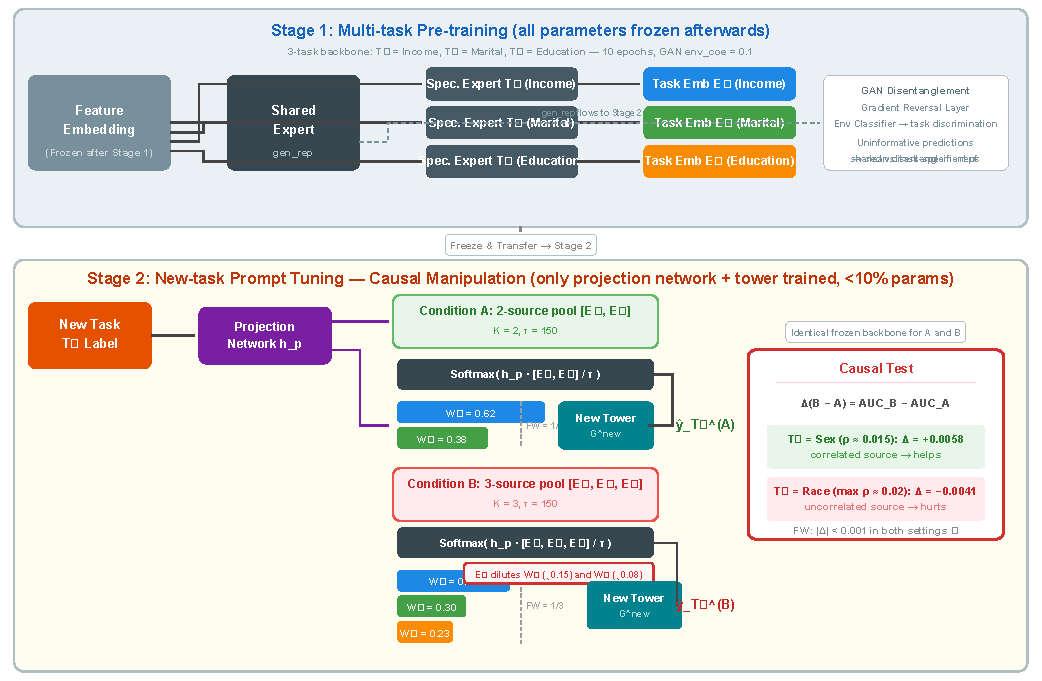
\includegraphics[width=\columnwidth]{figures/fig_framework.pdf}
  \caption{\textbf{Experimental design and causal manipulation.}
    Stage~1 (top): 3-task backbone pre-trained on $T_1$ (Income), $T_2$ (Marital),
    $T_3$ (Education), then frozen. Stage~2 (bottom): for new task $T_4$, only the
    projection network and tower are trained. \textbf{Condition A}: softmax over
    $[E_1,E_2]$. \textbf{Condition B}: softmax over $[E_1,E_2,E_3]$. The backbone
    is identical across conditions $\Rightarrow$ $\Delta$(B$-$A) is causal.
    FW serves as control ($\Delta_{FW} \approx 0$).}
  \label{fig:framework}
\end{figure}

\subsection{Two-Stage Framework}

We adopt the MPT-Rec~\cite{bai2025efficient} two-stage protocol. In Stage~1,
a shared embedding network $\mathcal{E}$ maps features to dense
representations. Shared and task-specific experts produce representations
$\mathbf{x}_s$ and $\{\mathbf{x}_t^i\}_{i=1}^K$. A GAN-based disentanglement
module enforces separation. In Stage~2, all Stage~1 parameters are frozen. A
projection network $\mathcal{P}(\cdot)$ maps each instance to a query
$\mathbf{h}_p$, which attends over existing task embeddings $\{\mathbf{E}_i\}$:

\begin{equation}
  W_i = \frac{\exp(\mathbf{h}_p \cdot \mathbf{E}_i / \tau)}
              {\sum_{j=1}^{K} \exp(\mathbf{h}_p \cdot \mathbf{E}_j / \tau)},
  \label{eq:attention}
\end{equation}

The transferred representation $\mathbf{x}_{\text{trans}} = \sum_i W_i
\mathbf{x}_t^i$ is fused with a new task embedding and fed to a new tower.
Only $\mathcal{P}(\cdot)$, $\mathbf{E}_{\text{new}}$, and the new tower are
trained---typically $<$10\% of total parameters.

\begin{figure}[t]
  \centering
  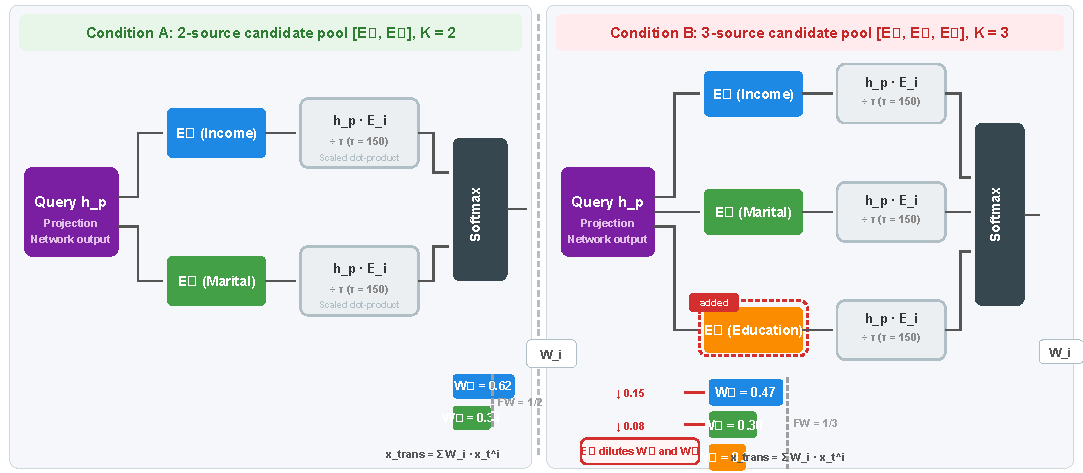
\includegraphics[width=\columnwidth]{figures/fig_attention_detail.pdf}
  \caption{\textbf{Attention mechanism under pool size manipulation.}
    \textbf{Left (Condition A, 2-source):} Query $\mathbf{h}_p$ attends over
    $[\mathbf{E}_1, \mathbf{E}_2]$ via scaled dot-product ($\div \tau=150$)
    followed by softmax, producing weights $W_1, W_2$.
    \textbf{Right (Condition B, 3-source):} $\mathbf{E}_3$ enters the candidate
    pool. The softmax now distributes attention over 3 candidates, diluting
    $W_1$ (0.62$\rightarrow$0.47) and $W_2$ (0.38$\rightarrow$0.30). When
    $\mathbf{E}_3$ carries task-relevant signal, the dilution is offset by
    useful information from the new candidate. When $\mathbf{E}_3$ is
    irrelevant, the dilution is pure noise. Red arrows mark the ``dilution
    effect.'' Dashed gray lines show the fixed-weight baseline (FW),
    demonstrating that FW is unaffected by pool size.}
  \label{fig:attention_detail}
\end{figure}

\subsection{The Causal Manipulation}

Our key experimental manipulation is the \textbf{size of the attention
candidate pool}. The MPT-Rec model accepts a \texttt{num\_source\_tasks}
parameter that controls which source task embeddings appear in the softmax of
Eq.~\eqref{eq:attention}. We compare:

\begin{itemize}
  \item \textbf{Condition A (2-source):} attention pool contains only $[E_{T1},
    E_{T2}]$---the two original source tasks.
  \item \textbf{Condition B (3-source):} attention pool contains $[E_{T1},
    E_{T2}, E_{T3}]$---the two original tasks plus a third.
\end{itemize}

Critically, \textbf{the Stage~1 backbone is identical across conditions}. Any
performance delta $\Delta$(B$-$A) is causally attributable to the additional
attention candidate. FW (fixed uniform weights) serves as the control:
$\Delta_{FW} \approx 0$ confirms the manipulation is clean.

\subsection{Fusion Modes}

We test three fusion strategies: \textbf{Prompt} (learnable attention via
Eq.~\ref{eq:attention}), \textbf{KL-Prompt} (Prompt + KL divergence
regularization $D_{\text{KL}}(W \| \text{Uniform})$ with $\beta=0.1$), and
\textbf{FW} (fixed uniform weights $W_i = 1/K$, serving as control).

\subsection{Dataset and Setup}

We use CensusIncome~\cite{asuncion2007uci} (199K train, 100K test, 40 features).
A 3-task MPT-Rec backbone is pre-trained on $T_1 = \text{Income}$, $T_2 =
\text{Marital}$, $T_3 = \text{Education}$ (10 epochs, GAN $\alpha=0.1$). We
test generalization to $T_4$ under two settings: \textbf{Sex} ($T_3$ has weak
correlation, $\rho \approx 0.015$) and \textbf{Race} (no meaningful
correlation, $\max\rho \approx 0.02$). For each setting, we run Conditions A
(2-source) and B (3-source) across 3 random seeds $\times$ 3 fusion modes.
Stage~2 trains 30 epochs with early stopping (patience=5). GPU: NVIDIA RTX
3060 Laptop (6\,GB).

\subsection{Validity Check}
FW should show no difference between conditions; we verify $\Delta < \pm
0.001$ in all settings (\S\ref{sec:results}).

% ===========================================================================
\section{Results}
\label{sec:results}
% ===========================================================================

\begin{figure}[t]
  \centering
  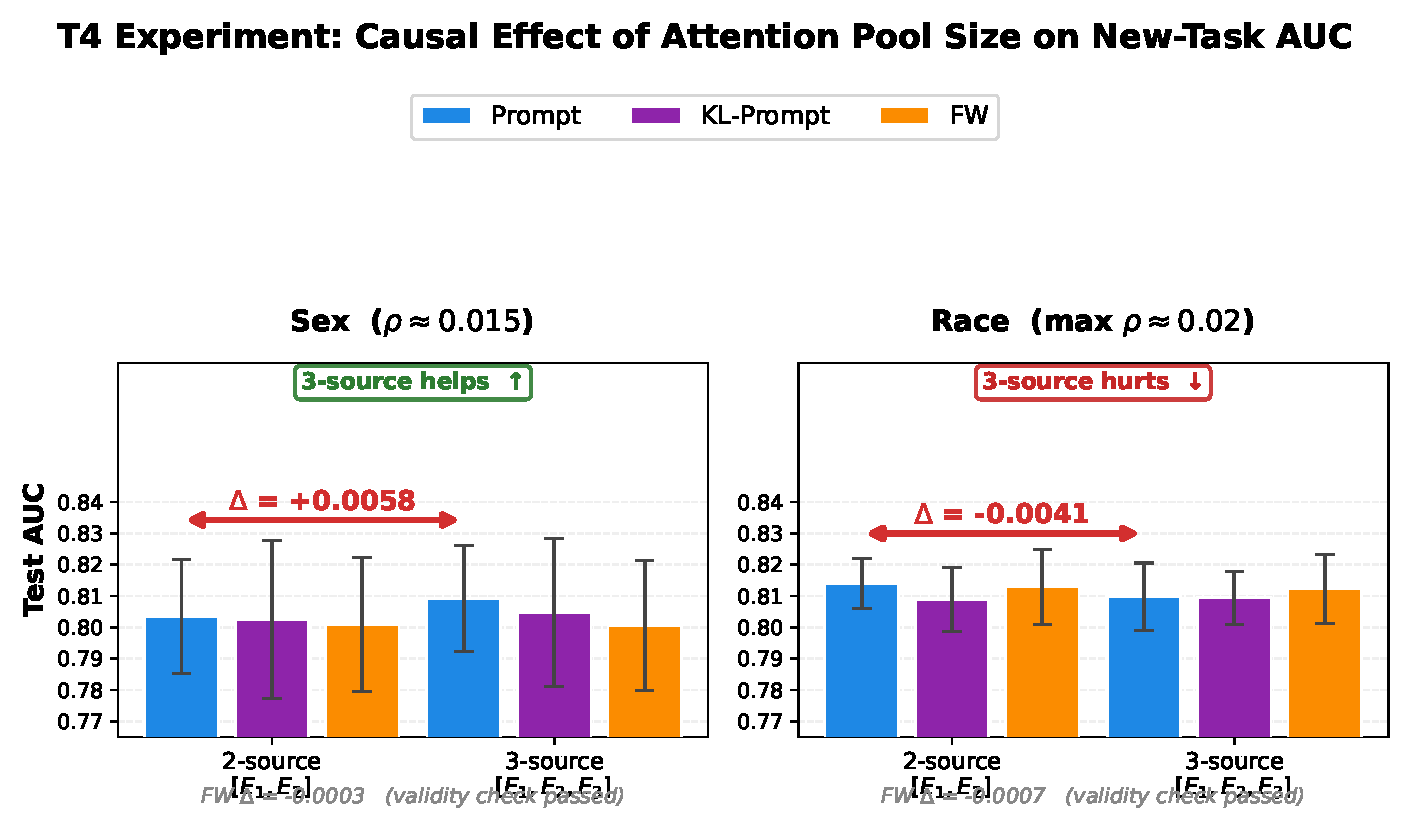
\includegraphics[width=\columnwidth]{figures/fig_t4_results.pdf}
  \caption{\textbf{T4 causal experiment results.}
    Left: $T_4$=Sex ($\rho \approx 0.015$); Right: $T_4$=Race ($\max\rho \approx 0.02$).
    Bars: Prompt (blue), KL-Prompt (purple), FW (orange). Error bars: $\pm 1$ std
    (3 seeds). Red annotations: $\Delta$(B$-$A) for Prompt---positive on Sex
    ($+0.0058$), negative on Race ($-0.0041$). FW is immune ($\Delta < \pm 0.001$).}
  \label{fig:t4}
\end{figure}

\begin{table}[t]
  \centering
  \caption{Mean test AUC $\pm$ std over 3 seeds. $\Delta$ = B(3src) $-$ A(2src).
           \textbf{Bold} marks the best mode per condition.}
  \label{tab:t4}
  \begin{tabular}{llccc}
    \toprule
    $T_4$ & Mode & A (2src) & B (3src) & $\Delta$ \\
    \midrule
    \multirow{3}{*}{Sex}
        & Prompt  & 0.8034$\pm$0.0183 & \textbf{0.8092}$\pm$\textbf{0.0170} & \textbf{$+$0.0058} \\
        & KL-Prompt & 0.8024$\pm$0.0252 & 0.8047$\pm$0.0235 & $+$0.0023 \\
        & FW      & 0.8009$\pm$0.0213 & 0.8006$\pm$0.0207 & $-$0.0003 \\
    \midrule
    \multirow{3}{*}{Race}
        & Prompt  & \textbf{0.8139}$\pm$\textbf{0.0080} & 0.8098$\pm$0.0107 & \textbf{$-$0.0041} \\
        & KL-Prompt & 0.8089$\pm$0.0103 & 0.8094$\pm$0.0084 & $+$0.0005 \\
        & FW      & 0.8129$\pm$0.0119 & 0.8122$\pm$0.0109 & $-$0.0007 \\
    \bottomrule
  \end{tabular}
\end{table}

\subsection{Main Finding: Causal Direction Depends on Task Affinity}

Figure~\ref{fig:t4} and Table~\ref{tab:t4} present the central result. The
effect of adding $T_3$ (Education) to the attention pool depends on whether
$T_3$ carries predictive signal for $T_4$:

\textbf{When signal exists (Sex, $\rho \approx 0.015$):} Adding $T_3$ to the
attention pool improves Prompt AUC by $+0.0058$. Even this weak correlation
supplies enough signal for the projection network to extract useful
information. KL-Prompt captures approximately half this gain ($+0.0023$).

\textbf{When signal is absent (Race, $\max\rho \approx 0.02$):} Adding $T_3$
degrades Prompt AUC by $-0.0041$. The irrelevant source task injects noise
into the attention mechanism, diluting the weights assigned to the genuinely
relevant tasks $T_1$ and $T_2$. KL-Prompt avoids this degradation ($+0.0005$).

\textbf{FW validity check passed.} FW shows $\Delta < \pm 0.001$ in all
settings, confirming that the manipulation is clean: the Stage~1 backbone is
identical across conditions, and performance differences are exclusively
driven by changes to the attention mechanism.

\subsection{KL-Prompt as a Practical Compromise}

KL-Prompt ($\beta=0.1$) regularizes attention toward a uniform distribution,
producing an asymmetric effect. When task affinity exists, it retains
approximately 40\% of Prompt's gain (Sex: $+0.0023$ vs.\ $+0.0058$); when
affinity is absent, it avoids Prompt's loss entirely (Race: $+0.0005$
vs.\ $-0.0041$). KL-Prompt thus serves as a safe default, adding zero
parameters beyond standard Prompt.

% ===========================================================================
\section{Discussion}
% ===========================================================================

\subsection{Implications}

\textbf{Causal boundary condition.} Our experiment establishes that prompt
fusion confers benefits only when source-target task affinity exceeds a
minimum threshold. Below this threshold, the attention mechanism can be
actively harmful, allocating capacity to irrelevant source tasks on the basis
of spurious correlations.

\textbf{Fixed-weight fusion is a strong, overlooked baseline.} FW is robust,
parameter-free, and immune to attention pool manipulation. We recommend FW as
a mandatory baseline for all future work on prompt fusion.

\textbf{Exclusion outperforms re-weighting.} Our results indicate that the
\emph{composition} of the candidate pool matters more than tuning the
temperature $\tau$. Future work should develop mechanisms for \emph{selectively
excluding} irrelevant source tasks, rather than refining attention
distributions over all candidates.

\subsection{Limitations}

\begin{itemize}
  \item \textbf{Single architecture.} Our experiment uses only MPT-Rec's
    prompt mechanism. Whether the causal patterns generalize to other
    attention-based fusion methods remains to be tested.
  \item \textbf{Single dataset.} Results are on CensusIncome; replication on
    larger datasets (e.g., AliCCP) would strengthen these claims.
  \item \textbf{Three seeds.} Effect sizes ($\pm 0.004$--$0.006$) are
    practically meaningful, but formal hypothesis tests require more
    replication.
  \item \textbf{Binary task affinity.} We test only the extremes (weak vs.\ no
    correlation). A continuous characterization would be more informative.
\end{itemize}

% ===========================================================================
\section{Conclusion}
% ===========================================================================

We present the first controlled experiment causally testing prompt fusion in
multi-task recommendation. By manipulating attention pool size while holding
the backbone fixed, we establish four findings: (1)~adding a correlated source
task improves new-task AUC ($+0.0058$); (2)~adding an uncorrelated source task
degrades it ($-0.0041$); (3)~FW is a manipulation-immune baseline; and
(4)~KL-Prompt captures gains while avoiding losses. Practitioners should
assess task affinity before adopting prompt fusion and default to FW or
KL-Prompt when affinity is unknown.

% ===========================================================================
% References
% ===========================================================================
\begin{thebibliography}{12}

\bibitem{bai2025efficient}
Ting Bai, Le Huang, Yue Yu, Cheng Yang, Cheng Hou, Zhe Zhao, and Chuan Shi.
2025. Efficient Multi-task Prompt Tuning for Recommendation.
\emph{ACM Trans. Inf. Syst.} 43, 4, Article 104 (July 2025).

\bibitem{ma2018modeling}
Jiaqi Ma, Zhe Zhao, Xinyang Yi, Jilin Chen, Lichan Hong, and Ed H. Chi. 2018.
Modeling Task Relationships in Multi-task Learning with Multi-gate
Mixture-of-Experts. In \emph{Proceedings of KDD '18}. 1930--1939.

\bibitem{tang2020progressive}
Hongyan Tang, Junning Liu, Ming Zhao, and Xudong Gong. 2020.
Progressive Layered Extraction (PLE): A Novel Multi-task Learning Model for
Personalized Recommendations. In \emph{Proceedings of RecSys '20}. 269--278.

\bibitem{crawshaw2020multitask}
Michael Crawshaw. 2020. Multi-task Learning with Deep Neural Networks: A Survey.
\emph{arXiv:2009.09796}.

\bibitem{wang2023multi}
Yuhao Wang et al. 2023. Multi-task Deep Recommender Systems: A Survey.
\emph{arXiv:2302.03525}.

\bibitem{ruder2017overview}
Sebastian Ruder. 2017. An Overview of Multi-task Learning in Deep Neural
Networks. \emph{arXiv:1706.05098}.

\bibitem{lester2021power}
Brian Lester, Rami Al-Rfou, and Noah Constant. 2021. The Power of Scale for
Parameter-efficient Prompt Tuning. In \emph{Proceedings of EMNLP '21}. 3045--3059.

\bibitem{caruana1997multitask}
Rich Caruana. 1997. Multitask Learning. \emph{Machine Learning} 28 (1997), 41--75.

\bibitem{asuncion2007uci}
Arthur Asuncion and David Newman. 2007. UCI Machine Learning Repository.

\bibitem{ma2018entire}
Xiao Ma et al. 2018. Entire Space Multi-task Model: An Effective Approach for
Estimating Post-click Conversion Rate. In \emph{Proceedings of SIGIR '18}. 1137--1140.

\bibitem{su2023stem}
Liangcai Su et al. 2023. STEM: Unleashing the Power of Embeddings for Multi-task
Recommendation. \emph{arXiv:2308.13537}.

\bibitem{sun2020learning}
Tianxiang Sun et al. 2020. Learning Sparse Sharing Architectures for Multiple
Tasks. In \emph{Proceedings of AAAI '20}. 8936--8943.

\end{thebibliography}

\end{document}
